\documentclass[letter]{article}

\usepackage[english]{babel}
\usepackage[utf8]{inputenc}
\usepackage{amsmath}
\usepackage{graphicx}
\usepackage[colorinlistoftodos]{todonotes}
\usepackage[top=1.5in, bottom=1.5in, left=1.5in, right=1.5in]{geometry}

\title{Results Addendum: Evolutionary Design of Particle Swarms}

\author{Benjamin Bengfort, Kevin Harrison, Phillip Kim}

\date{\today}

\begin{document}
\maketitle

Our second experiment consisted of changing the evolutionary computation mechanism slightly to make the search space more consistent. Instead of including one elite in the next generation, we carried five elites over. We also revised our mutation operator code to ensure that it was mutating in small, linear steps. Finally, we implemented recombination to try to allow genetic material from elites to influence the entire population. 

Our second experiment used 50 individuals per population and ran for 100 generations. With the revised code, you can see in Figure \ref{fig:meanfit} that our experiment converged after approximately 50 generations. The best individual was discovered in population 97, but the maximum fitness individuals were also very close and consistent after 50 generations. This was a much better result than our first evolutionary computation experiment which had extremely variable mean fitness and the each generation exhibited much different behavior than their parent generation.

\begin{figure}
	\centering
	    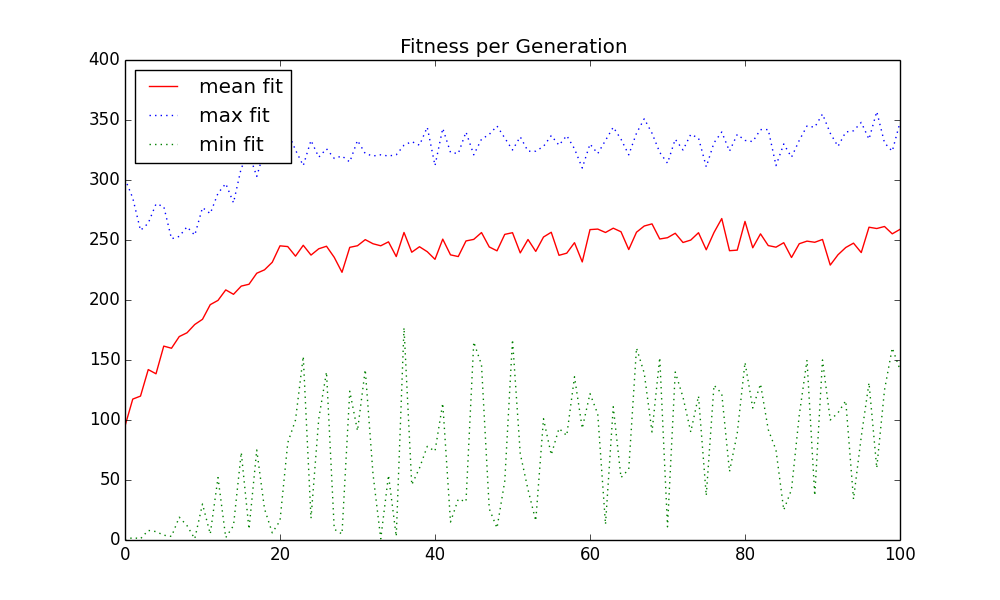
\includegraphics[width=0.75\textwidth]{figures/meanfit_experiment2}
    \caption{\label{fig:meanfit}Fitness per generation}
\end{figure}

The best evolved particle not only exhibited swarm behavior, but performed significantly better at the locate and collect task than the human designed particle. We compared the performance of both the evolved and human designed particles vs. a human designed particle by running each simulation 32 times then computing the mean resources in the home base of each team at every timestep. Further, we extended the maximum timesteps for the simulation from 10,000 (used to determine fitness) to 20,000 to see if any different behavior resulted and to ensure that the swarms had enough time to collect all the resources. 

As illustrated in Table \ref{table:meanfitness}, the evolved swarm collected over 100 more resources on average than the human designed swarm, with a significantly lower standard deviation. Averaged across all timesteps, Figure \ref{fig:head2head} shows the performance of the human designed vs human designed and evolution designed vs human designed swarms. Competing against each other, the human design swarms do equivalently in competition. However the evolution designed swarm is able to not only capture more resources faster, but around timestep 7000, begins to steal resources from the enemy base on average. 

Qualitatively, the evolved swarm exhibits a very different spreading behavior than the human designed swarm. As exhibited in Figure \ref{fig:spreading} the evolved particles spread more radially, able to explore more of the world earlier on. Another characteriation of this is the size of the swarm, which is much larger, but then breaks apart into smaller swarms once resources are discovered, in order to better exploit more resources deposits at once. In contrast, the human designed particles tend to stay in one or two larger flocks and only exploit one depot at a time.

\begin{table}
    \renewcommand{\arraystretch}{1.5}
    \centering
    \begin{tabular}{l | c c cc}
        \hline
        Simulation & Mean & Std Dev & Max & Min \\
        \hline
        human vs human & 249.125 & 42.618 & 319 & 177 \\
        evolved vs human & 397 & 4.833 & 400 & 386 \\
        \hline
    \end{tabular}
    \caption{Fitness of particles competing against human designed particle.}
    \label{table:meanfitness}
\end{table}

\begin{figure}
\centering
\begin{minipage}{0.5\textwidth}
	\centering
    	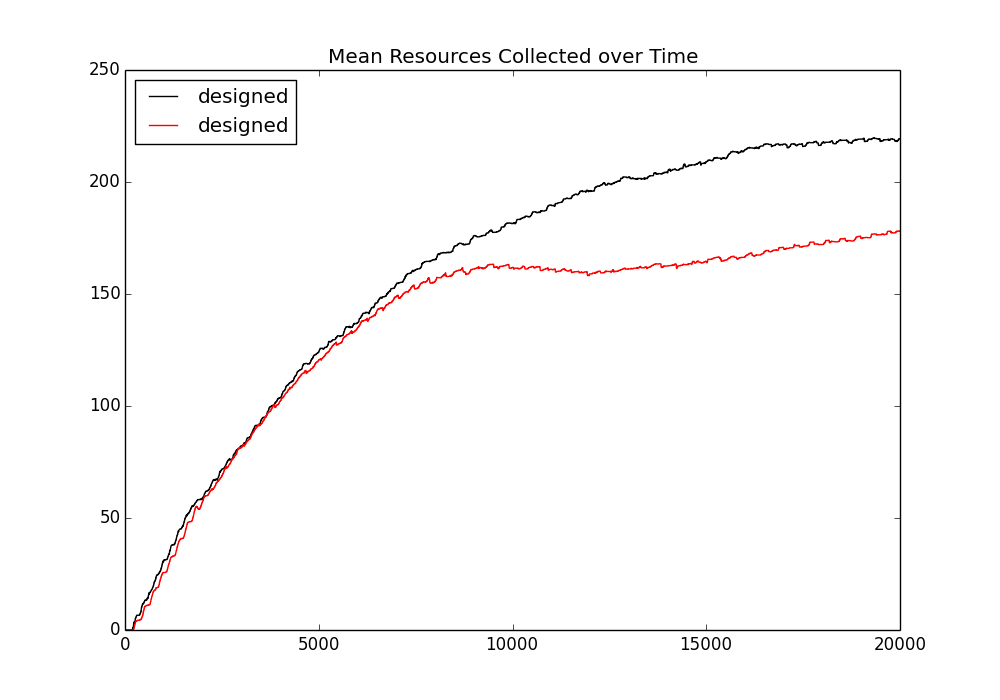
\includegraphics[width=\textwidth]{figures/designed_v_designed}
\end{minipage}%
\begin{minipage}{0.5\textwidth}
	\centering
    	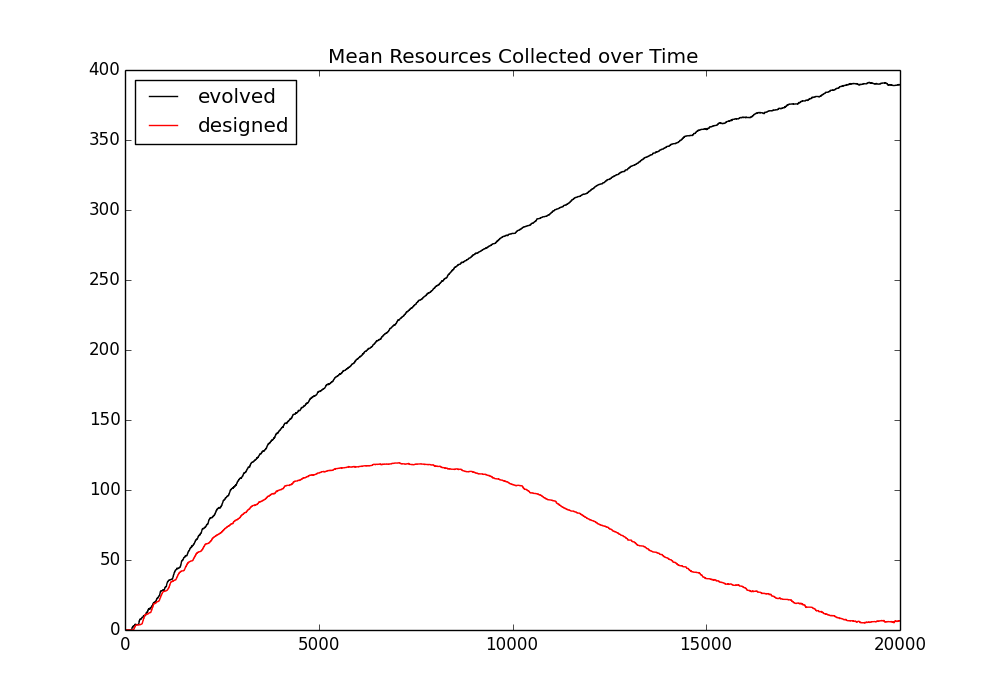
\includegraphics[width=\textwidth]{figures/evolved_v_designed}
\end{minipage}
	\caption{\label{fig:head2head}Evolution Designed vs Human Designed Swarms}
\end{figure}

\begin{figure}
	\centering
    	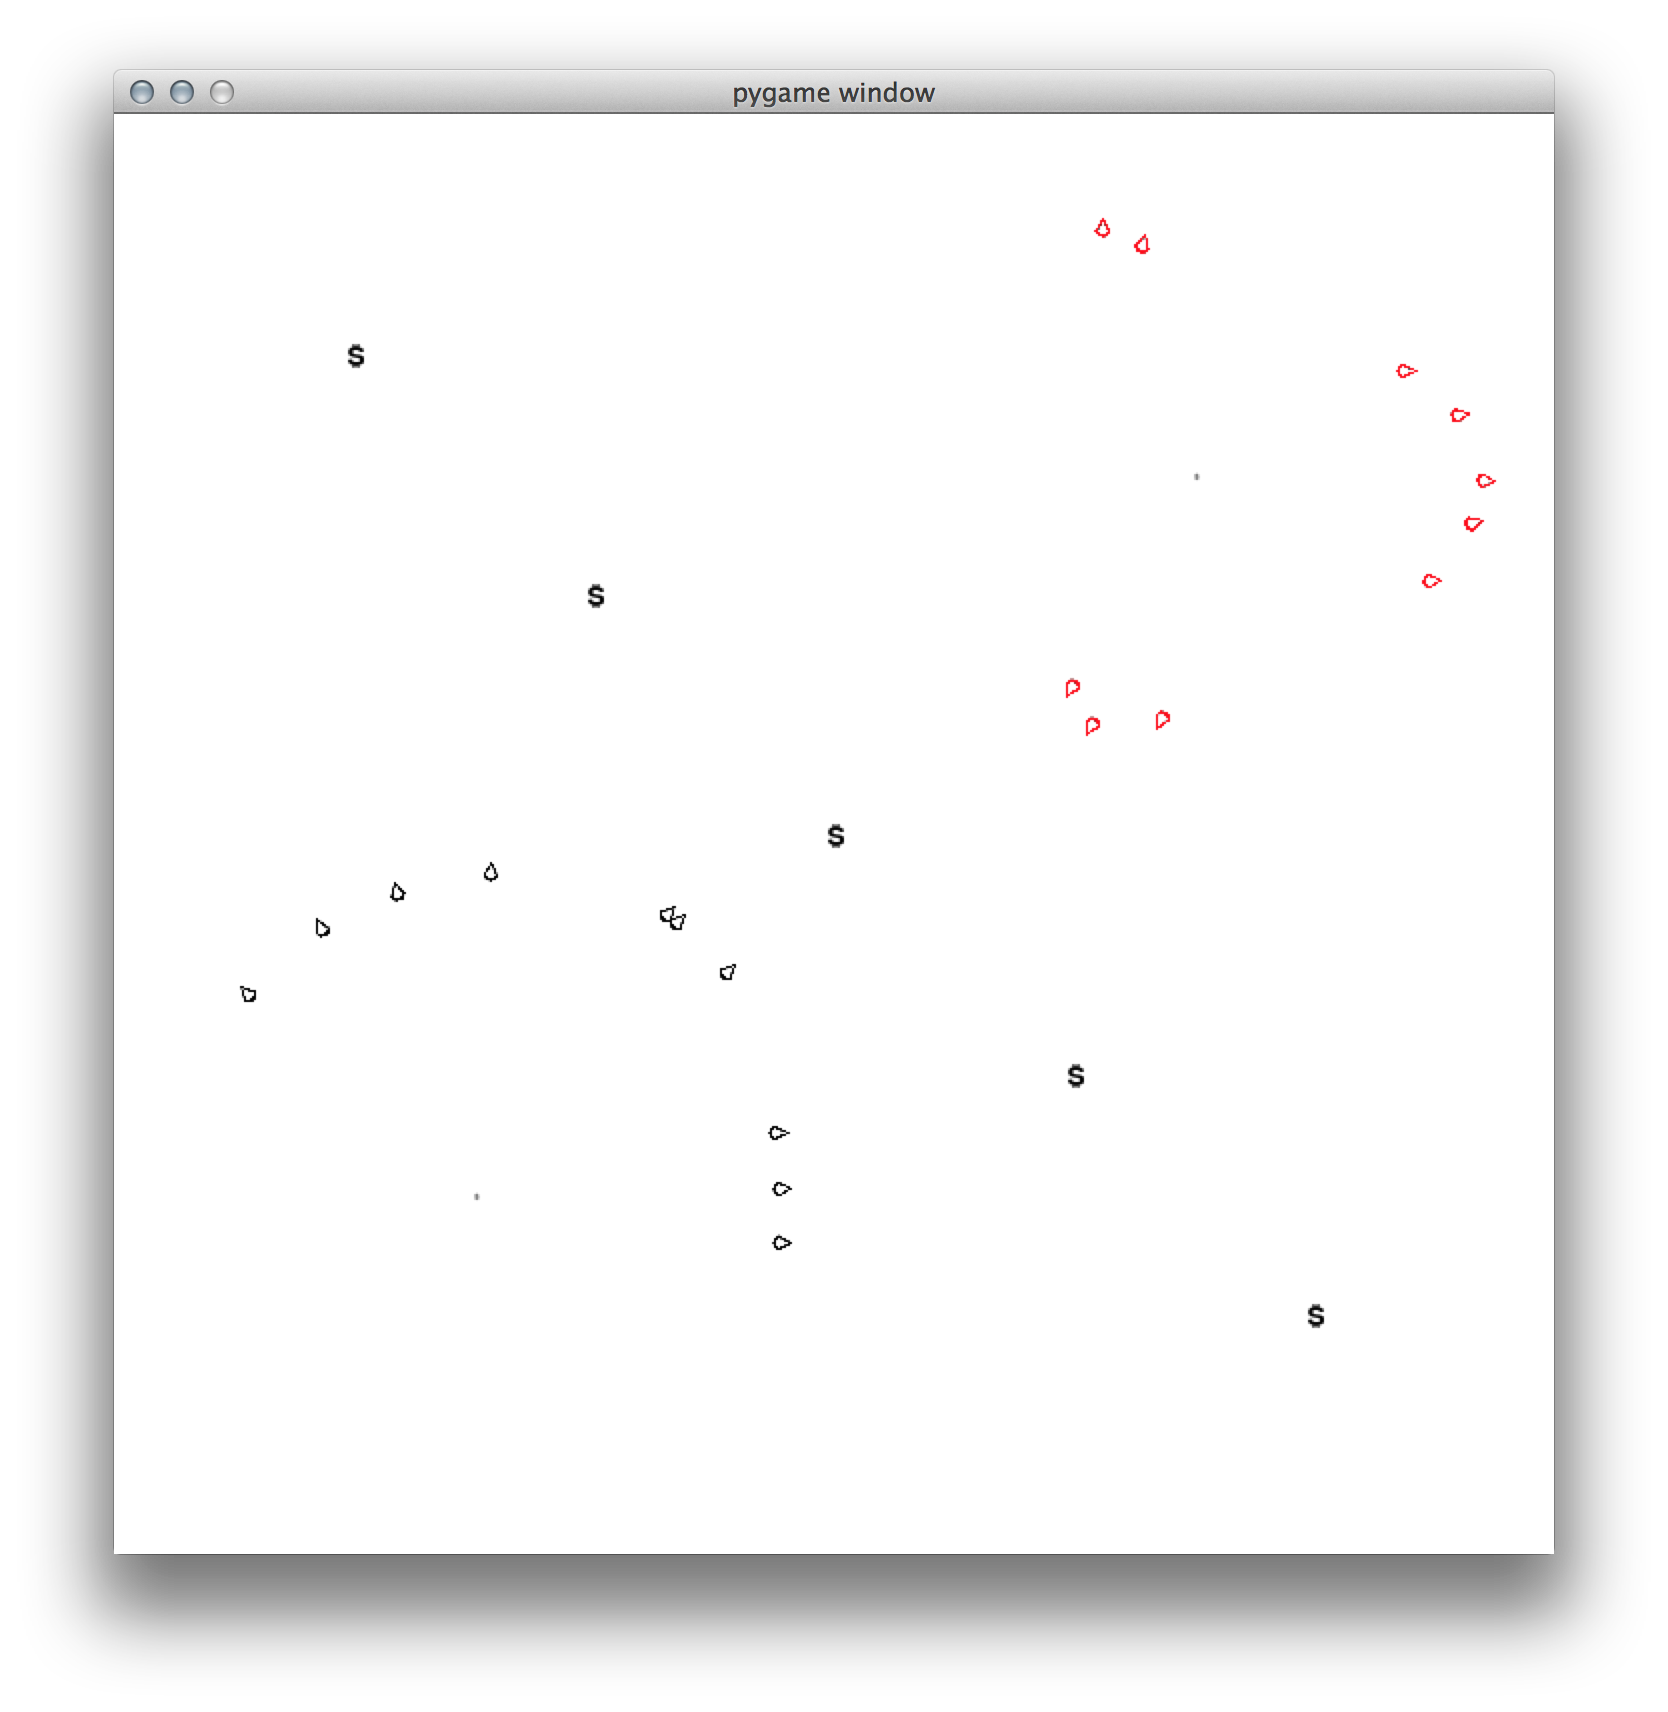
\includegraphics[width=0.75\textwidth]{figures/spreading}
    \caption{\label{fig:spreading}Spreading behavior of two types of swarms.}
\end{figure}

\end{document}